\section{Resource Management}

\subsection{Overview}

Resource Management in the HPC space has historically taken
numerous and varied forms. From early batch schedulers to
recent thrusts into Grid computing, the resource management
sphere has a dizzying breadth of work and research. Due to this
volume of research and data the term {\em resource management} is
unfortunately not well defined, so we take the opportunity here
to explicitly define resource management in the \ngrm\ system.

In this document, we define resource management as the management
of the state, topology information, access and utilitization
of all resources configured in \ngrm. The Resource Manager (RM)
component of \ngrm\ acts as the arbiter of efficient utilization
of these resources by accepting user requests for resources and
creating a schedule for these resource requests based on site
policy. The \ngrm\ RM is the user's portal to the resources
management by the system.

One of the main goals of \ngrm\ is to create a RM system
that is {\em extensible}, {\em scalable}, and {\em
generalized}(\ref{ReqsHiLevFun}). To meet these goals, we
build our resource manager on a set of components that are
themselves extensible and generalized. It is intended that
these components form a framework upon which a useful RM
subsystem is implemented. The core components of this system,
which are described in detail below, include a set of global,
persistent databases called the {\em Resource Inventory} and
{\em Job} and {\em User Repositories}, which contain the global
configuration of resources, users, and historical job data. Within
an \ngrm\ job, these databases are not persistent, and are instead
implemented as lightweight versions called simply the {\em resource
database} (RDB), {\em job database} (JDB), and {\em user database}
(UDB). Running within a job, we call a functioning collection of
these databases, and the interface to them a \ngrm\ {\em instance}.
(See Figure~\ref{RMInstance}).


\begin{figure}
\centering
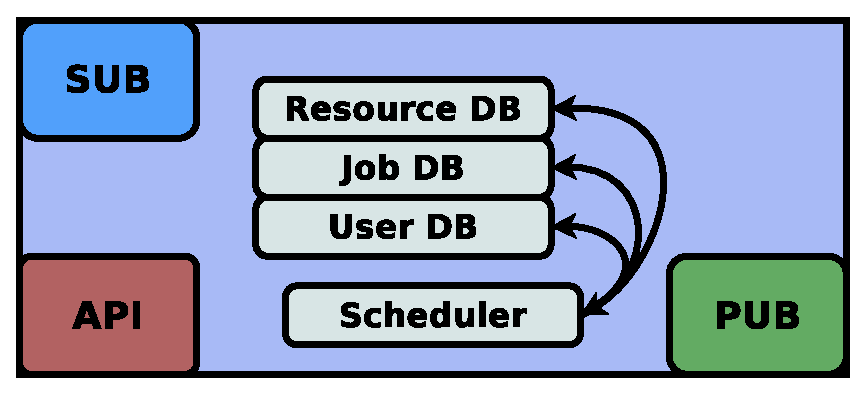
\includegraphics[scale=0.30]{../fig/RM-instance.eps}
\caption{Components of a Resource Manager Instance}
\label{RMInstance}
\end{figure}

A high level view of these components is presented in Figure~\ref{RMComponents}.

\begin{figure}
\centering
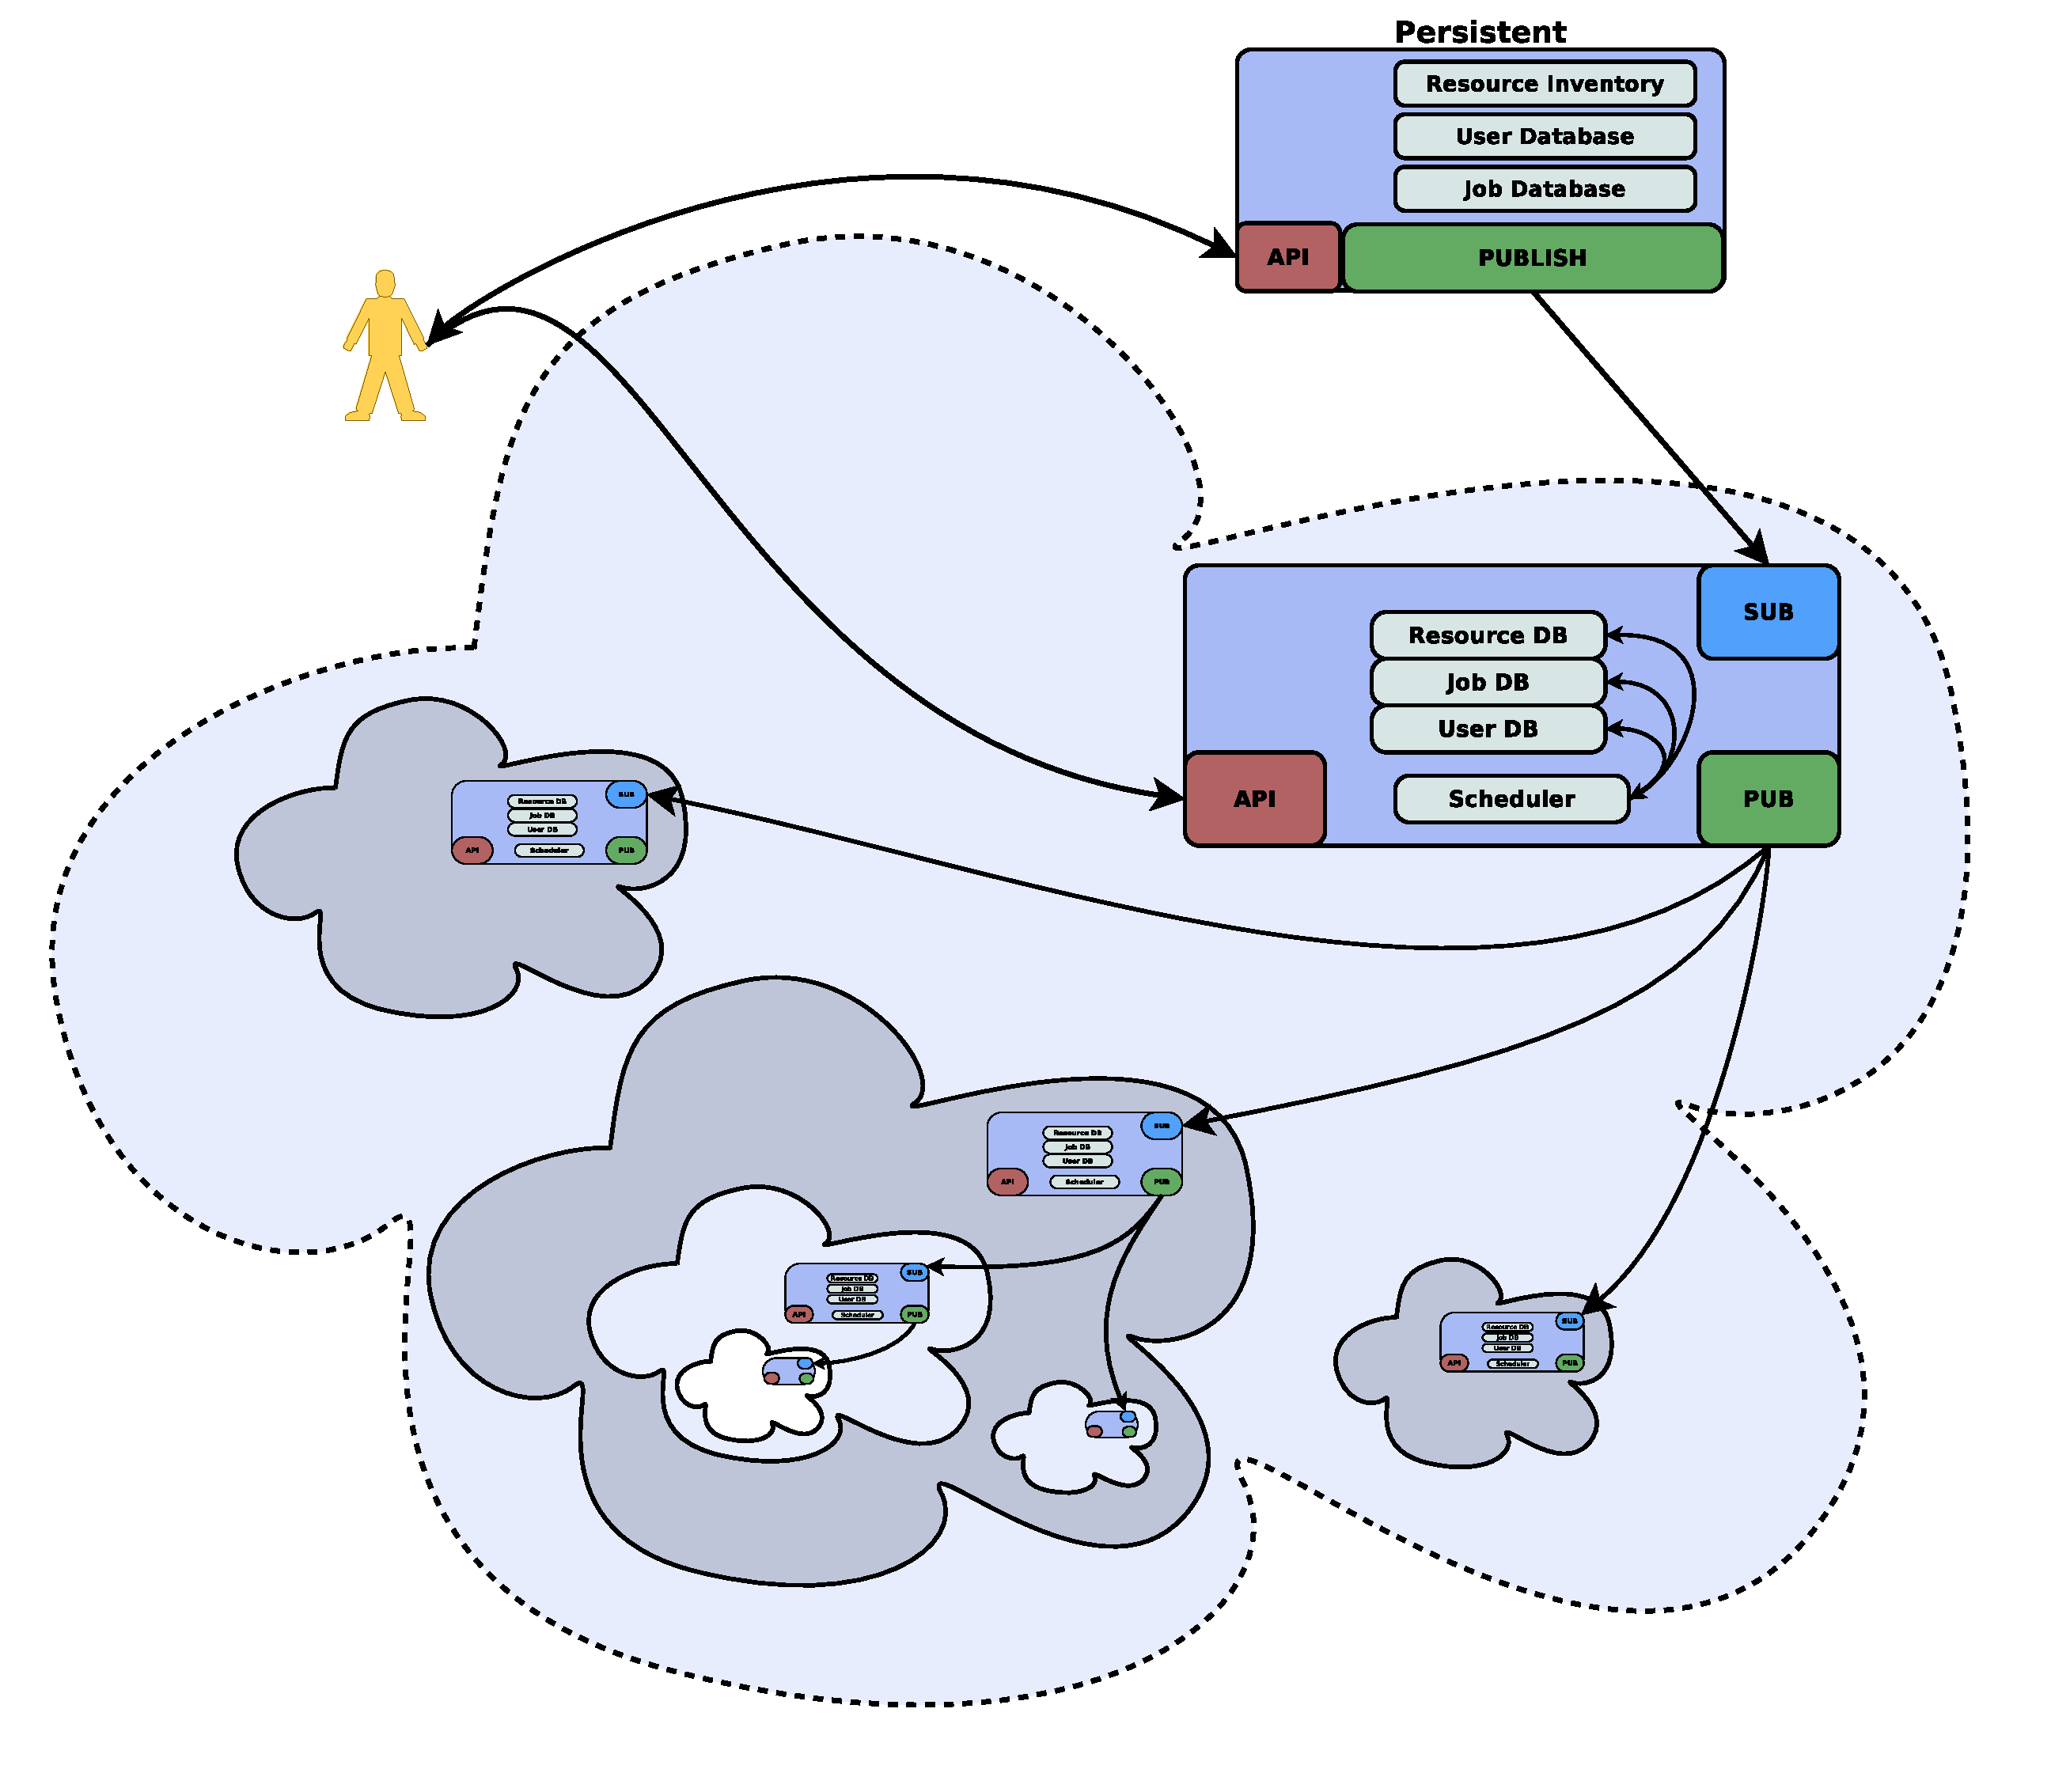
\includegraphics[scale=0.20]{../fig/RM-full.eps}
\caption{Resource Manager High Level View}
\label{RMComponents}
\end{figure}

In \ngrm\ users requesting resources, administrators configuring
or operating on resources, or subsystems utlizing resources
must have a flexible and extensible method for describing those
resources.  To meet this goal we introduce the idea of a {\em
resource description language} (RDL) in the sections below. We
also discuss a similar {\em job description language} (JDL) which
is used to encode generic job information in \ngrm. In \ngrm\
we consider that the Resource DB and Inventory {\em speak} RDL
and the Job DB and Repository {\em speak} JDL.

Finally, with these components in place, we discuss how we will
build a {\em Scheduler} in \ngrm. The Scheduler is a core component
of an \ngrm\ instance as it is responsible for building the schedule
that maps resource requests to time slots and resources, and thus
implements the essential functionality of the system -- that is the
efficient use of limited resources across a diverse user base while
implementing site policy.

\subsection{Resource Inventory}
\label{sect:resdb}

The core component of the resource management system is
a persistent, global database called the {\em resource inventory}.
The resource inventory contains a superset of resources managed
by the system, and at the highest level acts as the configuration
repository for the NGRM system.

The resource inventory, which is not associated with any instance
of the resource manager, will have the following initial features:

\begin{itemize}
\item{Arbitrary "tagging" of resource objects. Tags can be used later
   to define searches for objects. E.g. give me all the resources
   with the tag 'compute' and 'node' and 'idle', etc.}

\item{A subscribe interface with filtering so apps using the DB can
   subscribe to interesting changes and updates in the DB.}

\item{An API upon which sysadmin and other tools could be developed.}
\end{itemize}

Resource manager instances/jobs do not interact directly with
the resource inventory.  Instead, each RM instance has associated
with it a rw "cache" of its subset of the resource inventory DB,
which we will call simply the resource DB.  The resource DB
listens for changes of interest from its parent DB using
the subscribe interface, and additionally publishes its own
changes such that a parent/child or other application can
be notified of data changes to the cache (e.g. node is allocated
to sub-job, node is marked down, user pushes some tags of
interest into the cache).

At the end of a job, a configurable set of data in the
resource DB would be pushed back up to the parent. This
allows accumulated data and job/user specific tags from
each job to percolate back up the system, possibly all
the way to the persistent resource inventory.

The resource inventory will also capture the dynamic activity of
resources going in and out of service and contain an interface to the
monitoring component to help provide this information.

\subsection{Resource Description Language}

The resource description language is used to describe resources
in the resource inventory and in resource requests.
The resource description language should be generic but at the same
time useful.  Several projects have explored this area including
Condor's ClassAd language\cite{ClassAd},
OAR's resource description language\cite{Oar},
and Legion's\cite{LegionGrid}\cite{LegionRM} object-oriented approach.

The \ngrm\ resource description language should be developed with
input from stakeholders and should represent resources in our system as
well as define requests for those resources, and additionally be
\begin{itemize}
\item{\textbf{Human readable:} a sysadmin should be able to 'program up'
a collection of resources like a cluster with minimal
effort and the result should be understandable.}
\item{\textbf{Extensible:} allow development of functions that can be used
to simplify the complex definition of resources and requests.}
\item{\textbf{Fast:} parsing should not require lots of CPU or memory since
our system will be parsing this stuff on a very regular basis.}
\end{itemize}

A possible solution is to implement the
resource description language in Lua\cite{Lua} because this
little language is small, fast, and embarassingly easy to embed and
extend.  Lua's table data structure also lends itself very nicely to
expressing heirarchical data.

\subsection{Job Repository and Job Description}
\label{sect:jobdb}

User requests for computing resource allocations are saved as job
records to the job repository.  Like the resource description language
above, the form of the job record needs to capture the most generic
specifications yet be flexible enough to include machine-specific
attributes as well as complex conditions, dependencies, and even the
associated batch script.

Particular attention is needed to specify jobs within jobs.  There may
be a need for a distributed job repository such that higher level jobs
do not necessarily need to contain information on child jobs.

The persistence of the job repository starts when the job is first
submitted.  Job records are updated as jobs are prioritized into a
queue and move from a queued state, through a running state, to a
completed state and perhaps to an archived state.

Usage statistics will be available from the job repository.  Data from
the job repository and the resource inventory will provide a complete
picture of what jobs were running on what resources under what
conditions at every point in time.

\subsection{User Repository}

The user repository contains an ACL of users permitted to submit jobs
to the \ngrm.  This is where bank accounts and qualities of service
are defined along with the users associated with each.  Limits,
constraints, target shares, and policy rules are stored in this
repository.  The contents of this repository ultimately determine
which users can run on which resources under what conditions and
subject to what limitations and constraints.

\subsection{Repository Design}

The job and user repositories only exist at the same level as the
resource inventory. That is, since they are persistent, they cannot be
tied to any one "job". Instead, these are all global databases with
one a common API.  They are accessible from any job and/or user
workstation via globally routable server name and port for example.

Within any job, there is a "simpler" implementation of each of these
databases that we just call the (job-local) resource, user, and job
databases (as indicated in Figure~\ref{RMComponents}).  In this case,
these databases are instantiated on an as needed basis, and they may
be implemented as rw cache of the same databases in the parent. In
this case, "instance 0" has a parent of the global, persistent
databases -- the resource inventory, and job and user repo.

All of these components provide a pub/sub interface such that children
watch for interesting changes in their parent, and parents watch for
interesting changes in the child. "Interesting" changes in this case
might be important data about resources in the child (this resource is
dead), or information about the child job itself (I'm dead).

We will adopt the model from UNIX process management and have the
parent instance "reap" its children. It is here that the job db from
the child can be "pulled" up from the child into the parent job db.
When instance 0 reaps jobs, this job data can be pushed up to its
parent, i.e. the persistent job repo.

(TBD -- how to store child job information in the parent such that the
historical lineage of the jobs and sub-jobs within the child are
preserved.  Maybe the reaping should be abstracted down in the comms
layer with callbacks to allow the higher level subsystems to reap
their analogs in children.)

In this model, historical job data makes its way up to the top-level
job repository as child jobs complete. Each "running" job instance has
information about its historical job lineage in its local job db, so
this information can also be queried directly from within the context
of a job. (e.g. in a DAT, if you want to only query information about
jobs from the DAT, you can query the DAT job instance. In fact,
information about jobs from the DAT are not populated to the top-level
job repository until the DAT "ends")

We will define how jobs indicate that they are "done" and need to be
reaped. A DAT "job" may need to be killed and reaped at the end of its
time limit. Normal batch jobs are complete when the batch script
running on the control node exits. A direct allocate/launch with WRAP
would be reaped when the processes being launched exit. (Any other
cases?)

(TBD -- What happens to an active job hierarchy when the top-level job
is killed?  What happens to pending job requests when a job is
terminated?  Killing a job might result in something like:

\begin{enumerate}
\item Freeze local job db (i.e. disallow new job submissions)
\item Terminate and reap children jobs
\item Kill local tasks
\end{enumerate}

Perhaps 2,3 could be swapped or done in parallel.)

\subsection{Job Scheduler}

The \ngjs\ is responsible for scheduling computing resources to users'
jobs.  Users submit to the scheduler requests for resources to run
their job.  The scheduler implements management's policy to decide
when and where to allocate the resources for each job.

This section presents the requirements for the \ngjs, a rough design
which meets those requirements, and a work breakdown structure for
developing the scheduler component.

\subsubsection{Motivation}

Scheduling batch jobs across a collection of networked computing
resources started in the 1990's with Livermore Computing's DPCS (later
known as LCRM).  It received users' job requests, selected a cluster
for each job, then dispatched the job to that cluster's resource
manager.  The Moab Workload Manager which replaced LCRM essentially
provided the same functionality.  And while SLURM provides some grid
functionality, it never matured enough to allow it to replace Moab for
production use.

The \ngjs\ will provide new functionality not available in any
commercial or open source project.  The \ngjs\ will schedule jobs
across resources in a computing center without regard to traditional
cluster boundaries.  A job will be able to request resources
containing a common feature (like connectivity to the same high speed
switch) or fitting within a limited power envelope.

In addition, the \ngjs\ will be designed to be recursive.  It will
have the capability to launch another instance of itself within the
context of a job.  The \ngjs\ will support plugin modules that provide
unique scheduling behavior and job prioritization.  Each recursive
instance of the scheduler will have the option to independently load
its own schdeuling plugin.  In so doing, the \ngjs's scheduling
capabilities will range from scheduling all resources in the center to
scheduling jobs on dedicated resources (DATs) to scheduling what were
formerly known as job steps.

Most importantly, the traditional boundaries between a job scheduler
and the resource manager will be redefined under \ngrm.  Instead of a
resource manager that manages every resource of a cluster, the
\ngrmfull\ will be instantiated on the fly by the \ngjs\ and manage
only the resources the scheduler allocates to the job (or recursive
job).

In order to continue to meet the needs of LC users, the \ngjs\ must
continue to provide all the services that Moab currently provides,
but...
\begin{itemize}
  \item More quickly and efficiently
  \item More accurately
  \item More reliably
  \item More easily
  \item More intuitively
  \item More flexibly
  \item More securely
  \item More transparently
  \item And require minimal intervention and oversight
\end{itemize}

\subsubsection{Requirements}

While a more detailed list of requirements is presented here
<ToBeDone>, the following provides an overview of the functionality
that the \ngjs\ will be expected to deliver.

\paragraph{Fundamental Requirements}

The following is the most definitive list of scheduling requirements.
A scheduler is not a scheduler unless it can do these:

\begin{itemize}
  \item Maintain current resource inventory including state, health
    and availability of all resources to be scheduled
  \item Receive job allocation requests
  \item Prioritize each job
  \item Schedule each job based on multiple resource requirements
  \item Backfill lower priority jobs whenever possible
  \item Allow for dynamic job growth and reduction
  \item Preempt running jobs to free up resources needed by higher priority jobs
  \item Provide status of all jobs with estimates of when each job will run
  \item Allow for recursive scheduling
\end{itemize}

\paragraph{Further Scheduler Requirements}

As part of its scheduling duties, the scheduler must also accommodate
user requests and provide versatile administration capabilities.

\begin{itemize}
  \item Respond to requests to hold, modify or cancel jobs
  \item Schedule jobs across the center
  \item Support complex job dependencies
  \item Restrict some operations based on roles
  \item Accept job reservations
  \item Originate and manage WRAP instances
  \item Dynamically adapt to configuration updates
  \item Save complete state and recover fully from a restart
\end{itemize}

\paragraph{Policy Enforcement}

The scheduler implements the center's policies for providing access to
its computing resources.  As part of this duty, the scheduler must

\begin{itemize}
  \item Reject job submissions for jobs which cannot or will never run
  \item Remove jobs that exceed time limits
  \item Enforce established limits on users, groups, projects (banks), etc
  \item Honor service level agreements and service quality requests
\end{itemize}

\paragraph{Organization Components}

The \ngjs\ functionality is broken down into the following components.
However it is designed, it must include the following facilities.

\textbf{Job Submission.} This the facility that receives a user's
request for a job allocation and adds a record of this request to
the job repository.  Each job submitted must be immediately rejected
if it cannot or is not allowed to run given the job specifications,
the resources available, and any restrictions in place.  Job
submission must be extremely fast and return a job ID in well under a
second of time.  The system shall support hundreds of job submissions
per second.

\textbf{Job Prioritization.}  This the facility for prioritizing jobs
based on potentially multiple factors.  The system shall offer a job
priority plugin framework to allow custom algorithms for determining
job priority.  The priority of each queued job must be continually
recalculated as the queue of jobs and constituent factors are
constantly changing.

\textbf{Job Scheduling.} For each job removed from the prioritized
queue, computing resources must be reserved and eventually allocated.
The collection of resources to schedule must be available from the
resource inventory with the state and status of each resource updated in
real-time.  The scheduler must honor multiple resource requests
simultaneously as it seeks to allocate cores, GPUs, nodes, switches,
bandwidth, power, etc.

Here too, the system shall offer a plugin framework to support custom
algorithms for scheduling jobs to compute resources.  An essential
scheduling algorithm which must be included is backfill scheduling
(lower priority jobs are scheduled to run if they do not delay the
start of higher priority jobs).  In addition, qualities of service must
be implemented in the scheduler such that running jobs can be
preempted if needed to free up resources for more important jobs.
This involves not only selecting the best resources for a job, but
also identifying the set of jobs to preempt when such a policy is
enforced.

The output of a the job scheduling process is a schedule of which jobs
are mapped to which resources over a future, rolling period of time.
A by-product of this schedule is a projected start time for every
queued job that is included in the schedule.

\textbf{Job Dispatching.} As time passes, the allocations described in
the schedule must be created.  Running jobs that exceed their wall
clock limit much be terminated and new jobs must be launched.
Provisions must be made to launch multiple jobs simultaneously (or
nearly simultaneously).

\textbf{Job Status Reporting.} This is the facility for showing the
user the status of their jobs and the job queue.  Job info must be
available immediately after job submission, as it is pending, while it
is running, and afterwards for a period to be determined.  The system
should support multiple status requests at a time and reply with a
second or two.  The system is designed to withstand denial of service
attacks - whether deliberate or accidental.

\textbf{Job and System Management.} This is the facility for manual
intervention: boosting job priorities, modifying job characteristics,
cancelling jobs, etc.  Modifying resource states does not have to be
part of this facility.

\subsection{Resource Management API}

\paragraph{User Services}
This is the API for user or administrator interaction with the \ngrm.

\begin{itemize}
\item{$job\_submit()$: Submit a job allocation request and return a
  job ID}
\item{$job\_modify(JobID)$: Modify a job allocation request}
\item{$job\_status(JobID)$: Return complete information about a job}
\item{$job\_cancel(JobID)$: Cancel a job allocation request}
\item{$queue\_show()$: Return the current queue of jobs}
\item{$schedule\_show()$: Return the complete schedule as last
  calculated}
\end{itemize}

In addition, the following API provides users and administrators the
ability to query and modify the resource inventory, subject to roles
and permissions.

\begin{itemize}
\item{$resource\_add(Resource)$: Add a resource to the resource inventory}
\item{$resource\_modify(Resource)$: Modify the status/state of resource}
\item{$resource\_status(Resource)$: Return the status/state of resource}
\item{$resource\_remove(Resource)$: Remove a resource from the resource inventory}
\item{$resource\_group\_add(Resource)$: Add a resource group (e.g., node partition) to the resource inventory}
\item{$resource\_group\_status(Resource\_group)$: Return the status of a resource group}
\item{$resource\_group\_modify(Resource\_group)$: Modify the status/state of a resource group}
\item{$resource\_group\_remove(Resource)$: Remove a resource group from the resource inventory}
\end{itemize}

Similarly, the following API provides users and administrators the
ability to query and modify records in the user repository, subject to
roles and permissions.

\begin{itemize}
\item{$user\_add(User)$: Add a user with ACL to the user repository}
\item{$user\_modify(User)$: Modify the status or ACL of user}
\item{$user\_status(User)$: Return complete information about a user}
\item{$user\_remove(User)$: Remove a user from the user repository}
\end{itemize}

\paragraph{Scheduler Requests and Subscriptions}
This is the API the scheduler calls to request or subscribe to records
from the resource inventory, and job and user repositories.

\begin{itemize}
\item{$resource\_request()$: Request all schedulable resources from
  the resource inventory}
\item{$resource\_subscribe()$: Subscribe to changes to all schedulable
  resources from the resource inventory}
\item{$job\_request()$: Request all jobs from the job repository}
\item{$job\_subscribe()$: Subscribe to changes to all jobs from the
  job repository}
\item{$user\_request()$: Request all users from the user repository}
\item{$user\_subscribe()$: Subscribe to changes to all users from the
  user repository}
\end{itemize}

\paragraph{Scheduler Directives}
These are the WRAP service primitives the scheduler calls to initiate,
modify, and terminate WRAP instances. (Described in
Section~\ref{sect:prim} below)

\begin{itemize}
\item{$alloc()$}
\item{$realloc()$}
\item{$release()$}
\item{$launch()$}
\item{$destroy()$}
\end{itemize}


%\newpage
\subsection{Resource Management WBS}

\begin{longtable}{|p{1cm}|p{10.2cm}|p{1cm}|p{1cm}|p{1.8cm}|}\hline
  \textbf{Item} & \textbf{Description}
                & \textbf{Deliv}\footnote{SD = software drop,
                        DR = design review, V = viewgraphs, D = document}
                & \textbf{Weeks} & \textbf{Depend} \\
  \hline
  \hline
  \multicolumn{5}{|l|}{2.1. \textbf{General Resource Management}} \\
  \hline
  2.1.1.& "Functional", high-level model for how the system above
         would work in \ngrm, including models for Resource Inventory,
          Job Data, Queues, Scheduling.
        & V
        & 
        & \\
  \hline
  \multicolumn{5}{|l|}{2.2. \textbf{Resource Database}} \\
  \hline
  2.2.1.& Resource and Job DB APIs (design and prototype).
        & DR
        & 
        & 2.1.1\\
  \hline
  2.2.2.& Resource Inventory (design and prototype)
        & DR
        & 
        & 2.1.1\\
  \hline
  2.2.3.& Job Repository (design and prototype)
        & DR
        & 
        & 2.1.1\\
  \hline
  2.2.4.& User Repository (design and prototype)
        & DR
        &
        & 2.1.1\\
  \hline
  2.2.5.& Comms integration
        & DR
        & 
        & 2.1.1.\\
  \hline
  2.2.6& Research existing work in resource description languages,
	  such as Condor's ClassAd language,
	  OAR's resource description language,
          Legion's object-oriented resource approach.
        & V
        & 
        & \\
  \hline
  2.2.7.& Design/Prototype resource description language.
        & DR
        & 
        & \\
  \hline
  \multicolumn{5}{|l|}{2.3. \textbf{Job Scheduler}} \\
  \hline
  2.3.1.& Scheduler (design and prototype)
        & DR
        & 
        & 2.1.1\\

  \hline
\end{longtable}
